\documentclass[12pt,compress,ngerman,utf8]{beamer}
\usepackage{ragged2e}
\usepackage[ngerman]{babel}
\usepackage{multicol}
\usepackage{animate}
\usepackage{xstring}
\usepackage[protrusion=true,expansion=true]{microtype}

\DeclareSymbolFont{extraup}{U}{zavm}{m}{n}
\DeclareMathSymbol{\varheart}{\mathalpha}{extraup}{86}
\DeclareMathSymbol{\vardiamond}{\mathalpha}{extraup}{87}

\title{Prinzipiell unlösbare Probleme}
\author{Ingo Blechschmidt}
\date{7. September 2016}

\usetheme{Warsaw}

\useinnertheme{rectangles}

\usecolortheme{seahorse}
\definecolor{mypurple}{RGB}{150,0,255}
\setbeamercolor{structure}{fg=mypurple}

\usefonttheme{serif}
\usepackage[T1]{fontenc}
\usepackage{libertine}

\setbeamertemplate{navigation symbols}{}
\setbeamertemplate{headline}{}
\setbeamertemplate{frametitle}[default][colsep=-2bp,rounded=false,shadow=false,center]
\setbeamertemplate{blocks}[rounded][shadow=false]

\newcommand*\oldmacro{}%
\let\oldmacro\insertshorttitle%
\renewcommand*\insertshorttitle{%
  \oldmacro\hfill\insertframenumber\,/\,\inserttotalframenumber\hfill}

\newcommand{\hil}[1]{{\usebeamercolor[fg]{item}{\textbf{#1}}}}

\newcommand{\slogan}[1]{%
  \begin{center}%
    \setlength{\fboxrule}{2pt}%
    \setlength{\fboxsep}{6pt}%
    {\usebeamercolor[fg]{item}\fbox{\usebeamercolor[fg]{normal
    text}\parbox{0.7\textwidth}{\justifying#1}}}%
  \end{center}%
}

\begin{document}

\newcommand{\mytitlepage}{
  \centering
  % http://leverhawk.com/is-cloud-identity-an-unsolvable-problem-2012121599
  {\quad}
\includegraphics[scale=0.1]{unsolvable-problem}
  \bigskip

  \Large
  \hil{Prinzipiell unlösbare Probleme}
  \bigskip

  \scriptsize
  \insertauthor \\
  Linux User Group Augsburg e.\,V.
  \medskip

  \normalsize
  7. September 2016
  \par
}

\frame{\mytitlepage}

\frame{\frametitle{Alan Turing (* 1912, † 1954)}
  \centering
  % https://upload.wikimedia.org/wikipedia/commons/a/a1/Alan_Turing_Aged_16.jpg
  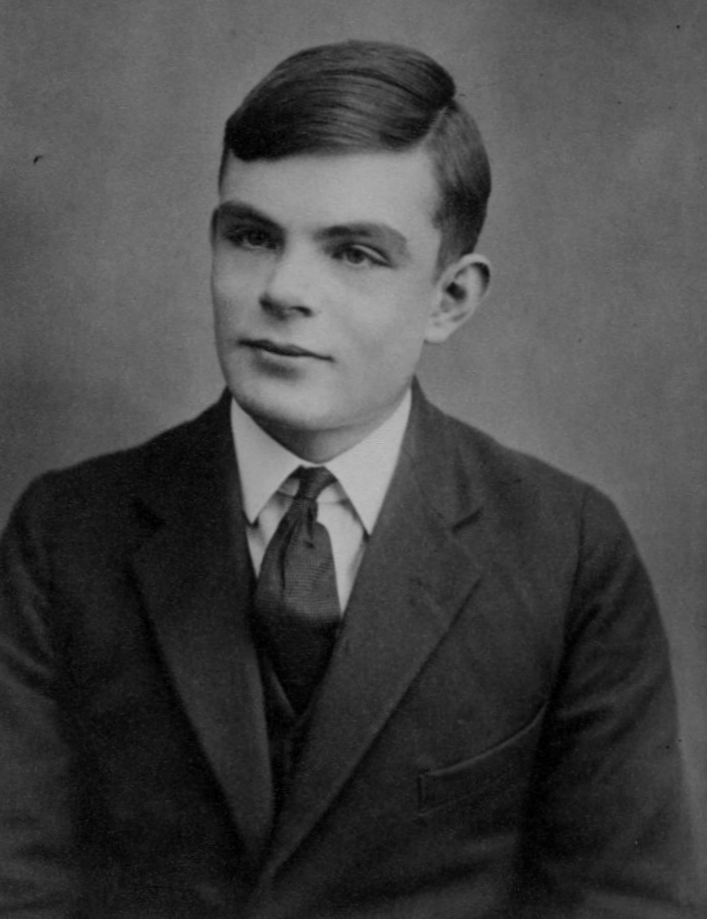
\includegraphics[width=0.5\textwidth]{alan-turing}
  \par
}

\frame{\frametitle{Turingmaschinen}
  \centering
  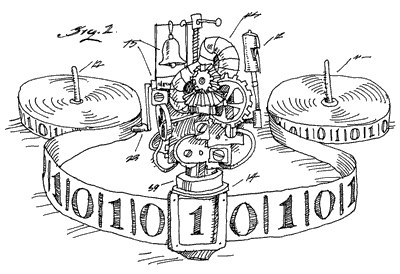
\includegraphics[width=0.7\textwidth]{turing-machine}
  \pause

  \bigskip
  Eine schwere Frage: \\
  \hil{Hält eine gegebene Turingmaschine?}
  \par
}

\frame{\frametitle{Brisanz des Halteproblems}
  \slogan{Wenn man jeder Turingmaschine ansehen könnte, ob sie schlussendlich
  hält, könnte man unzählige Probleme aus der Mathematik und den
  Naturwissenschaften lösen.}
  \pause
  \bigskip

  Zum Beispiel die \emph{Goldbachsche Vermutung}:
  \begin{center}Ist jede gerade Zahl größer als 2 die Summe zweier
  Primzahlen?\end{center}

  Die Primzahlen: $2, 3, 5, 7, 11, 13, 17, 19, 23, 29, 31, 37, \ldots$

  Für viele Zahlen stimmt's:
  \begin{align*}
    16 &= 11 + 5 \\
    124 &= 113 + 11 \\
    123456 &= 123449 + 7
  \end{align*}
}

\frame{\frametitle{Unlösbarkeit des Halteproblems}
  Toll wäre ein \hil{Halteorakel}: eine Maschine, die von einer gegebenen
  Maschine prüft, ob sie hält oder nicht.
  \pause
  \bigskip
  
  Wenn es ein Halteorakel gäbe, könnte man
  folgendes Programm schreiben:

  \begin{enumerate}
    \item Lese eine Zahl~$n$ vom Band als Eingabe ein.
    \pause
    \item Befrage das Halteorakel, ob das~$n$-te Programm (in einer Liste aller
    Programme) hält oder nicht.
    \pause
    \item Falls ja: Dann gehe in eine Endlosschleife.
    \item Falls nein: Dann halte an.
  \end{enumerate}
  \pause

  Dieses Programm kommt in der Liste aller Programme ebenfalls vor, sagen wir
  an~$m$-ter Stelle. Was passiert, wenn wir dieses Programm mit der Eingabe~$m$
  starten?
  
\includegraphics[height=0.7em]{trollface}
}

\end{document}
